\secnumbersection{DEFINICIÓN DEL PROBLEMA}

\subsection{Contexto}

En el mundo de la robótica existen diferentes categorías de competencias a lo largo del mundo. Una de las más antiguas es la All Japan Robotracer \& micromouse Contest\footnote{\url{https://www.ntf.or.jp/}, Página oficial de la competencia} con más de 40 años de trayectoria que consta de 2 categorías, Robotracer y Micromouse. 

Los objetivos de esta competencia son, por un lado, un punto de encuentro para desarrolladores, con un enfoque educativo, ya que se llama a participar a diferentes escuelas y universidades,y por el otro, es ser un cuna para la innovación, ya que diferentes empresas compiten acá para poner a pruebas nuevas tecnologías, y así evaluar su factibilidad y utilidad para luego poder implementarlas en aplicaciónes de la vida real. El enfoque de este trabajo va a ser en la categoría denominada Robotracer.

Las bases de la competencia de la categoría a trabajar son las siguientes: Se tiene una pista consistente de una linea blanca continua sobre fondo negro (Ver figura \ref{fig:pista1}). El robot debe ser capaz de recorrer la totalidad del trazado de forma válida, es decir, que la proyección del robot no se salga de este, y además detenerse por su cuenta. Esta pista no es conocida hasta el momento de participar, por lo que no se puede hacer un pre mapeado de la pista.

Se tienen 5 intentos dentro de un periodo de 3 minutos para lograr el menor tiempo posible. Lo normal es utilizar el primer intento para mapear la pista y los otros 4 para lograr vueltas válidas lo más rápido posible.

Aquí se puede ver la ronda del campeón actual de la competencia. \cite{ganador2023}

\begin{figure}[h]
\centering
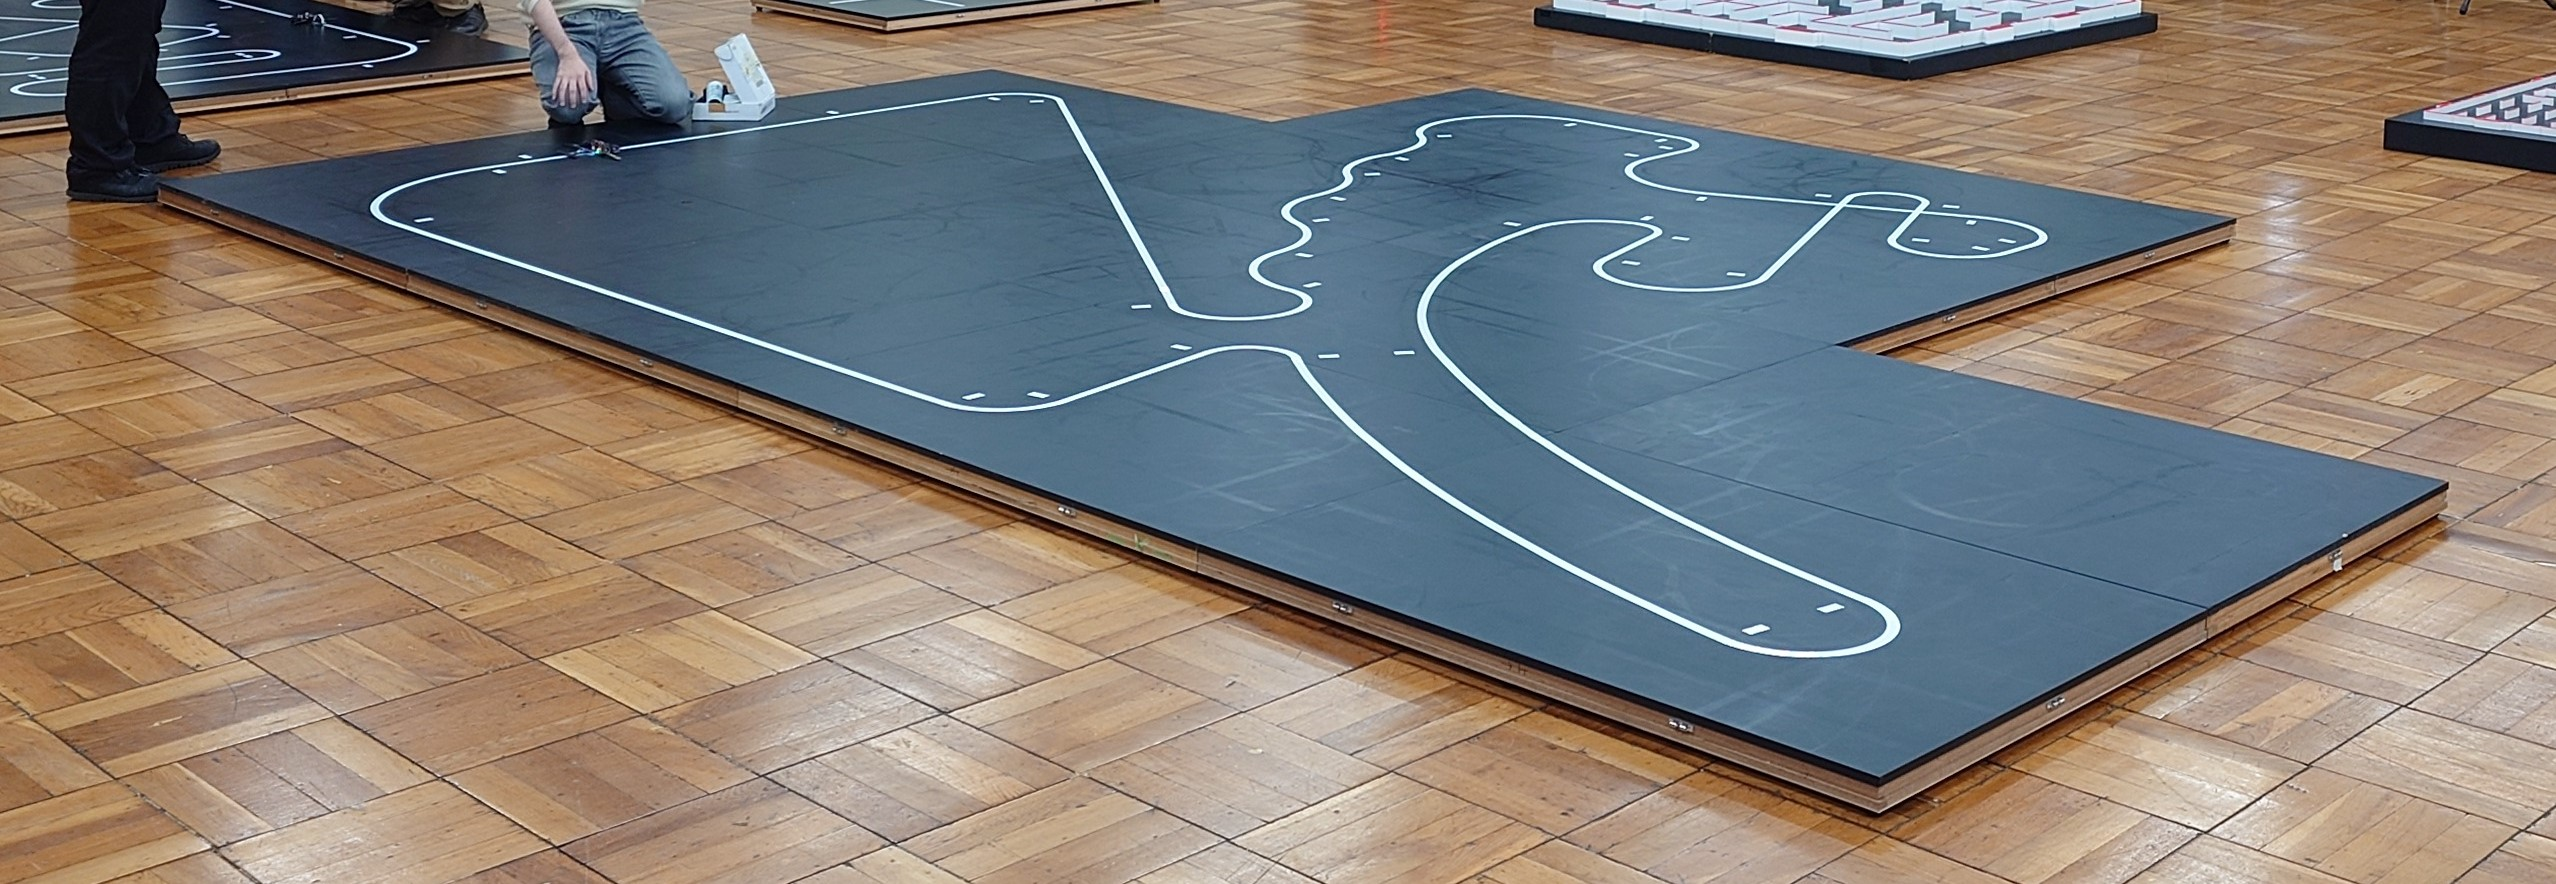
\includegraphics[width=0.8\textwidth]{ejemplo_pista_1}
\caption{\label{fig:pista1} Ejemplo de pista} Fuente: Elaboración propia.
\end{figure}

\subsection{Arquitectura Actual}
En la última competencia realizada, la gran mayoría (por no decir todos), programaba sus robots en C/C++, aplicando algoritmos de MATLAB (más adelante se detalla). La ventaja de esto es que MATLAB genera scripts en C/C++, por lo que se pueden usar algoritmos de optimización preexistentes sin mayores complicaciones.

\subsubsection{Seguimiento de línea}
El método actual para seguir la línea se basa principalmente en el uso de sensores infrarrojo para la obtención de la posición relativa del robot, y con esta información el uso de un PID para el control automático.

\subsubsection{Mapeo}
Para la primera vuelta, los robots deben ser capaces de las siguientes 2 características: identificar las marcas de curva que se encuentran en la pista en cada cambio de curvatura (Ver figura \ref{fig:marcaspista}) y poder saber su posición actual en términos de coordenadas cartesianas (x,y).

\begin{figure}[h]
\centering
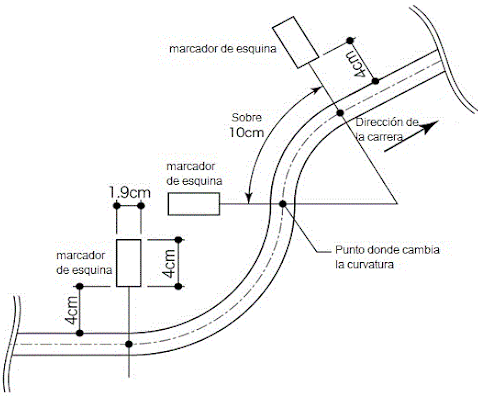
\includegraphics[width=0.5\textwidth]{ejemplo_marcas_curvas}
\caption{\label{fig:marcaspista} Ejemplo de marcas de curva} Fuente: All Chile Robot Contest.
\end{figure}

Para la primera, se necesitan sensores infrarrojos capaces de identificar blanco vs negro posicionados de tal forma que siempre detecten las marcas correspondientes. Para la segunda se pueden utilizar 2 elementos de manera independiente o junta (esta última es la más óptima): Encoders en cada rueda (Odometría), lo cual permite saber la velocidad real de cada una. Y una IMU , que básicamente es un giroscopio+acelerómetro.

De esta forma se puede hacer una estimación relativamente precisa de la posición del robot en términos de (x,y), resultando en una nube de puntos que representan la pista. Usualmente esta información es guardada en un simple txt.

\subsubsection{Optimización}
Con la nube de puntos generada, se utiliza un algoritmo de MATLAB conocido como PRM\footnote{\url{https://la.mathworks.com/help/robotics/ug/probabilistic-roadmaps-prm.html} , PRM algorithm.}, en donde se define 
un mapa binario donde la ruta generada, más el ancho del robot, se define como espacio válido para desplazarse, y el resto como obstáculo. Luego se generan puntos aleatorios dentro de la zona donde el robot puede pasar y finalmente se juntan los que permiten la ruta más corta posible(Ver figura \ref{fig:PRM}).

\begin{figure}[h]
\centering
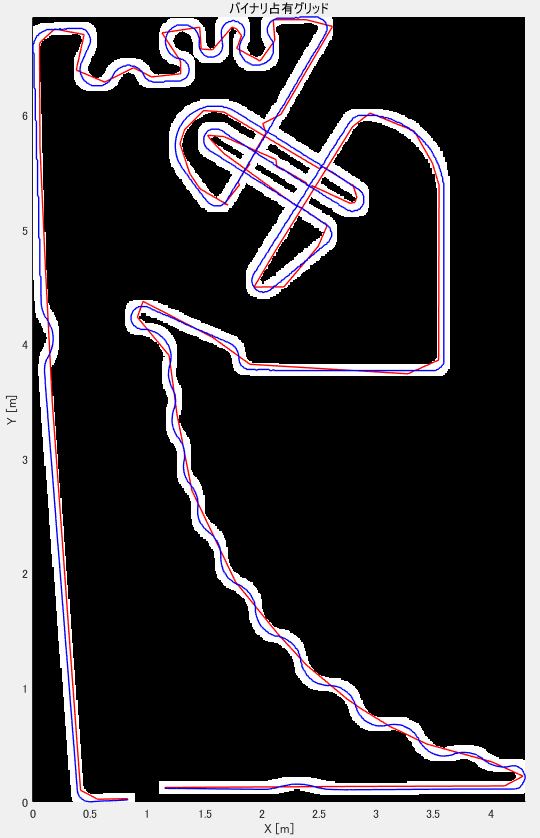
\includegraphics[width=0.5\textwidth]{ejemplo_optimizacion_PRM}
\caption{\label{fig:PRM} Aplicación de PRM} Fuente: Haruki Shimotori.
\end{figure}

\newpage
Con la ruta definida, mediante un algoritmo de seguimiento de rutas \footnote{\url{https://la.mathworks.com/help/robotics/ug/path-following-for-differential-drive-robot.html} , Path follower}, se le dan las instrucciones de movimiento al robot, donde en cada intento se varían las variables de velocidad, aceleración y freno.

Esta información fue basada en las publicaciones de Haruki Shimotori \footnote{\url{https://underbirdworks.blogspot.com/2020/12/matlabprm.html}, explicacion de Haruki Shimotori } y en el siguiente video se puede ver una idea similar en donde se utiliza Path Smoothing \cite{pathsmoothing}

\subsection{Información del problema}
Los últimos años todos los esfuerzos de mejora se han enfocado en la mecánica y electrónica del robot. dejando de lado el software. Estas mejoras van desde el uso de motores más potentes, más eficientes, sensores más precisos, mejoras en agarre y tracción del robot mediante turbinas, pero sin cambiar los algoritmos que hay por detrás.

Todas estas mejoras no se han considerado como innovaciones grandes, por lo que existe un espacio de investigación en el que el software pueda ser el protagonista. Es por este motivo que en la última versión no se ha otorgado el premio a la innovación a ningún participante, siendo su obtención uno de los objetivos de esta memoria.

\subsection{Objetivos}

\subsubsection{Objetivos Generales}

Implementar un método nuevo de seguimiento y mapeo de línea, para su posterior optimización enfocada en la maximización de la velocidad implementado en un robot sigue lineas,  mediante el uso de redes neuronales, específicamente visión computacional y aprendizaje reforzado. Estas redes neuronales van a estar trabajando en sincronía para lograr el mejor control en compentencia.

En primera instancia, se espera validar el trabajo mediante simuladores en diferentes disposiciones de pista, variando el nivel de dificultad, para eventualmente poder aplicar lo logrado con este trabajo en un robot real, que conste únicamente de un control diferencial de ruedas y una cámara, en la siguiente versión de la competencia All Japan para la verificación en un entorno competitivo de los métodos abordados.

\subsubsection{Objetivos específicos}

\begin{itemize}
	\item Implementar un algoritmo de visión computacional para un seguimiento exitoso de la pista en tiempo real.
	\item Implementar un algoritmo de mapeo de la pista en tiempo real, utilizando únicamente visión computacional.
	\item Implementar un algoritmo de aprendizaje reforzado para mejorar los tiempos entre intentos, optimizando el recorrido y velocidad a tiempo real.
	\item Desarrollar un simulador para realizar un pre-entreno de las redes neuronales involucradas.
	\item Desarrollar un robot sigue lineas para implementar los modelos anteriores en un entorno real.
\end{itemize}
\newpage
\subsection{Árbol del problema}

\begin{figure}[h]
\centering
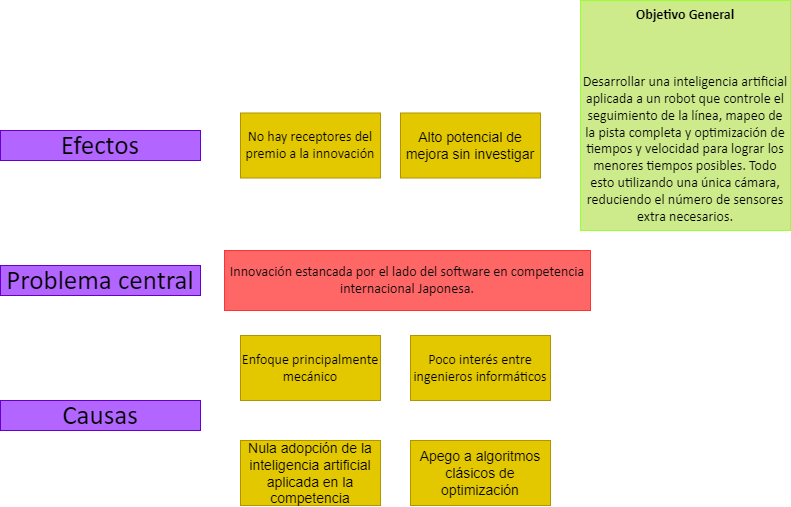
\includegraphics[width=1\textwidth]{diagrama_arbol}
\caption{\label{fig:arbol} Árbol del problema} Fuente: Elaboración Propia.
\end{figure}
